\documentclass{standalone}

\usepackage[utf8]{inputenc}
\usepackage[T1]{fontenc}
\usepackage{tikz}

\usetikzlibrary{shapes.geometric, arrows}

\tikzstyle{startstop} = [rectangle,
	rounded corners, 
	minimum width=3cm, 
	minimum height=1cm,
	text centered, 
	draw=black, 
	fill=red!30
	]

\tikzstyle{io} = [trapezium, 
	trapezium stretches=true,
	trapezium left angle=70, 
	trapezium right angle=110, 
	minimum width=3cm, 
	minimum height=1cm, 
	text centered, 
	draw=black,
	fill=blue!30
	]

\tikzstyle{choice} = [rectangle, 
	minimum width=3cm, 
	minimum height=1cm, 
	text centered, 
	text width=3cm, 
	draw=black, 
	fill=orange!30
	]

\tikzstyle{menu} = [diamond, 
	minimum width=3cm, 
	minimum height=1cm, 
	text centered, 
	draw=black, 
	fill=green!30
	]

\tikzstyle{arrow} = [thick,->,>=stealth]

\begin{document}

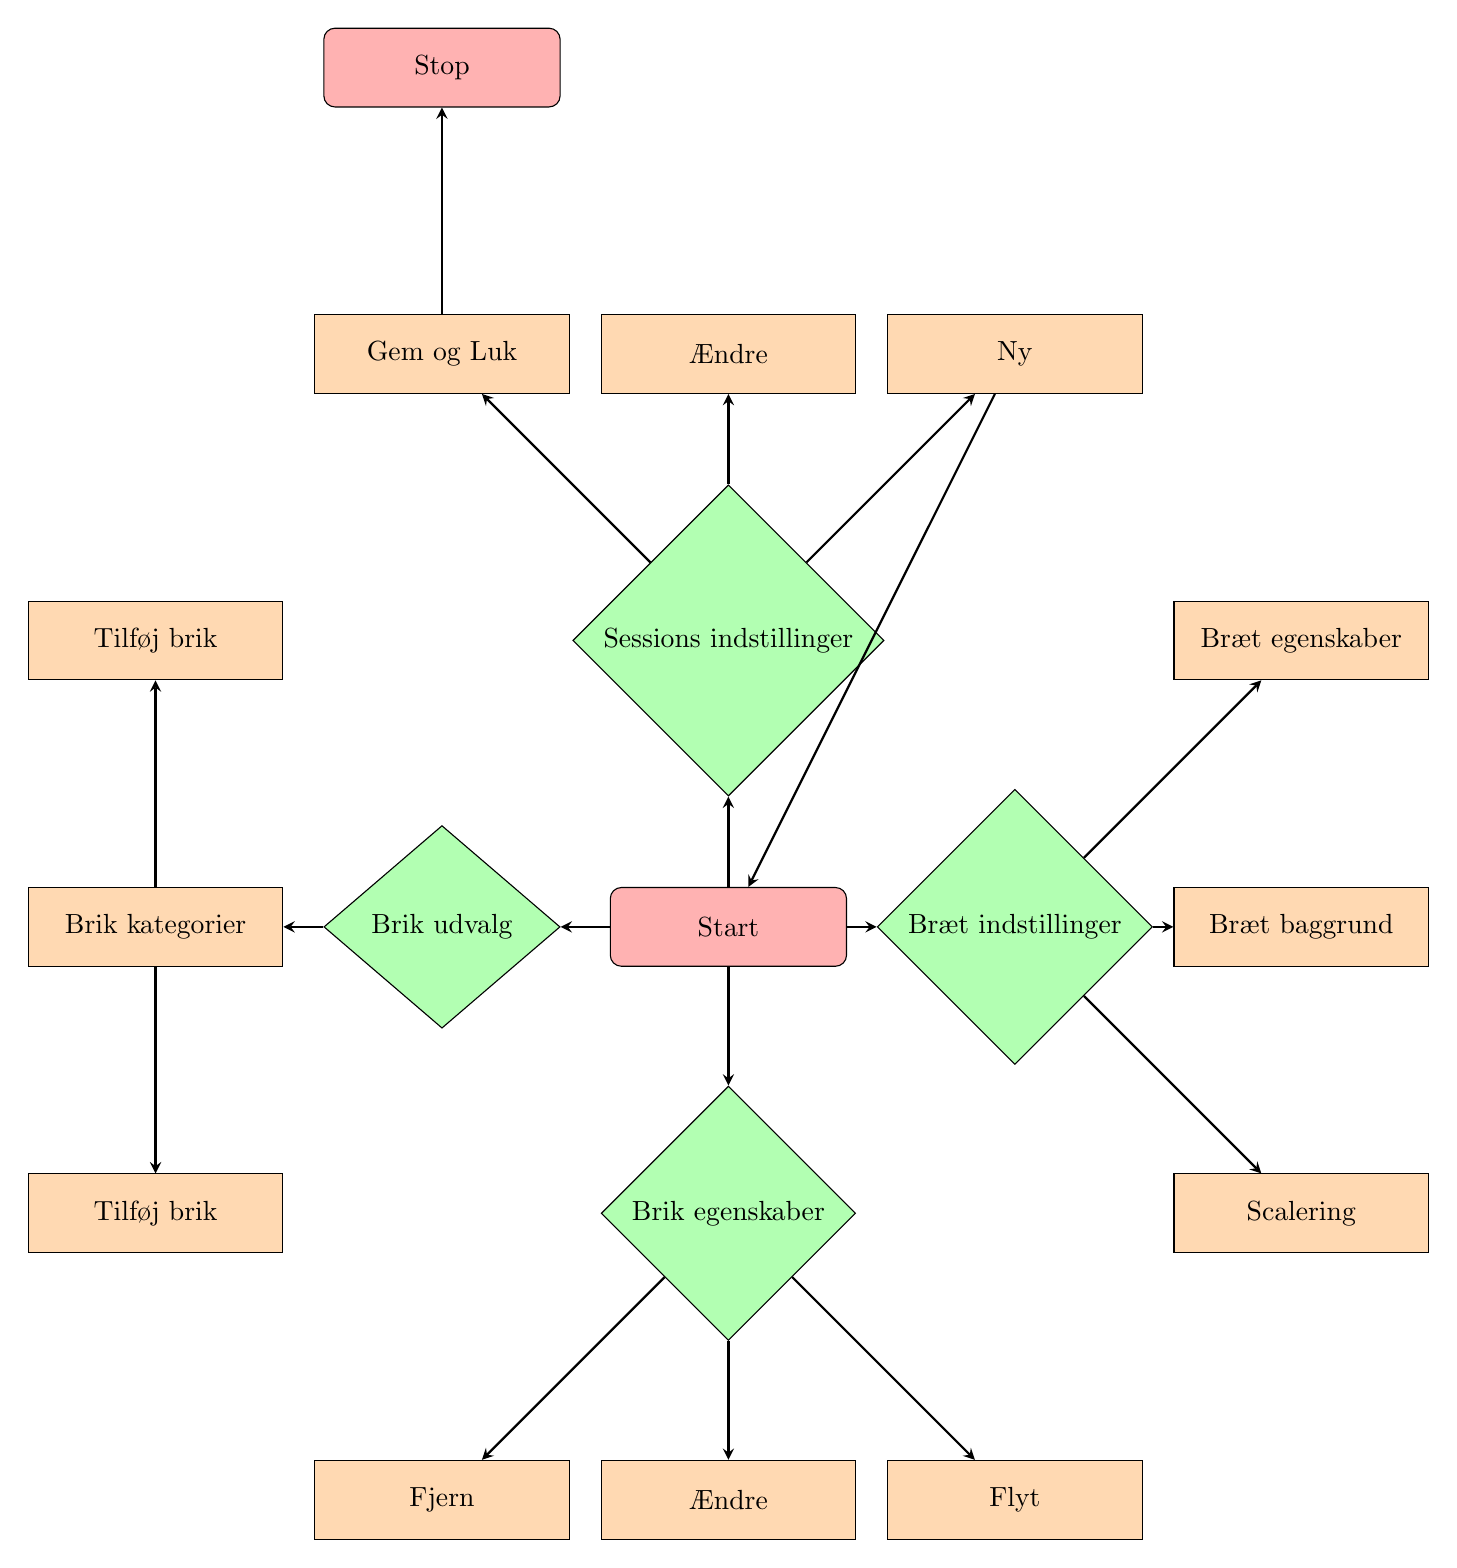
\begin{tikzpicture}[node distance=.3\textwidth]

\node (start) [startstop] {Start};
\node (mBE) [menu, below of=start] {Brik egenskaber};
\node (mBI) [menu, right of=start] {Bræt indstillinger};
\node (mSI) [menu, above of=start] {Sessions indstillinger};
\node (mBU) [menu, left of=start] {Brik udvalg};

\node (cSC) [choice, above of=mSI] {Ændre};
\node (cSS) [choice, left of=cSC] {Gem og Luk};
\node (cSN) [choice, right of=cSC] {Ny};

\node (stop) [startstop, above of=cSS] {Stop};

\node (cPC) [choice, below of=mBE] {Ændre};
\node (cPR) [choice, left of=cPC] {Fjern};
\node (cPM) [choice, right of=cPC] {Flyt};

\node (cTC) [choice, left of=mBU] {Brik kategorier};
%\node (cTI) [choice, left of=cTC] {vælg brik};
\node (cTIone) [choice, above of=cTC] {Tilføj brik};
\node (cTItwo) [choice, below of=cTC] {Tilføj brik};

\node (cBB) [choice, right of=mBI] {Bræt baggrund};
\node (cBP) [choice, above of=cBB] {Bræt egenskaber};
\node (cBS) [choice, below of=cBB] {Scalering};


\draw [arrow] (start) -- (mBE);
\draw [arrow] (start) -- (mBI);
\draw [arrow] (start) -- (mSI);
\draw [arrow] (start) -- (mBU);

\draw [arrow] (mSI) -- (cSC);
\draw [arrow] (mSI) -- (cSS);
\draw [arrow] (mSI) -- (cSN);

\draw [arrow] (cSS) -- (stop);
\draw [arrow] (cSN) -- (start);

\draw [arrow] (mBE) -- (cPC);
\draw [arrow] (mBE) -- (cPR);
\draw [arrow] (mBE) -- (cPM);

\draw [arrow] (mBU) -- (cTC);
%\draw [arrow] (cTC) -- (cTI);
\draw [arrow] (cTC) -- (cTIone);
\draw [arrow] (cTC) -- (cTItwo);

\draw [arrow] (mBI) -- (cBB);
\draw [arrow] (mBI) -- (cBP);
\draw [arrow] (mBI) -- (cBS);

\end{tikzpicture}

\end{document}